%%%%%%%%%%%%%%%%%%%%%%%%%%%%%%%%%%%%%%%%%
% Masters/Doctoral Thesis 
% LaTeX Template
% Version 2.5 (27/8/17)
%
% This template was downloaded from:
% http://www.LaTeXTemplates.com
%
% Version 2.x major modifications by:
% Vel (vel@latextemplates.com)
%
% This template is based on a template by:
% Steve Gunn (http://users.ecs.soton.ac.uk/srg/softwaretools/document/templates/)
% Sunil Patel (http://www.sunilpatel.co.uk/thesis-template/)
%
% Template license:
% CC BY-NC-SA 3.0 (http://creativecommons.org/licenses/by-nc-sa/3.0/)
%
%%%%%%%%%%%%%%%%%%%%%%%%%%%%%%%%%%%%%%%%%

%----------------------------------------------------------------------------------------
%	PACKAGES AND OTHER DOCUMENT CONFIGURATIONS
%----------------------------------------------------------------------------------------

\documentclass[
11pt, % The default document font size, options: 10pt, 11pt, 12pt
%oneside, % Two side (alternating margins) for binding by default, uncomment to switch to one side
english, % ngerman for German
singlespacing, % Single line spacing, alternatives: onehalfspacing or doublespacing
%draft, % Uncomment to enable draft mode (no pictures, no links, overfull hboxes indicated)
%nolistspacing, % If the document is onehalfspacing or doublespacing, uncomment this to set spacing in lists to single
%liststotoc, % Uncomment to add the list of figures/tables/etc to the table of contents
%toctotoc, % Uncomment to add the main table of contents to the table of contents
%parskip, % Uncomment to add space between paragraphs
%nohyperref, % Uncomment to not load the hyperref package
headsepline, % Uncomment to get a line under the header
%chapterinoneline, % Uncomment to place the chapter title next to the number on one line
%consistentlayout, % Uncomment to change the layout of the declaration, abstract and acknowledgements pages to match the default layout
]{MastersDoctoralThesis} % The class file specifying the document structure

\usepackage[utf8]{inputenc} % Required for inputting international characters
\usepackage[T1]{fontenc} % Output font encoding for international characters

\usepackage{mathpazo} % Use the Palatino font by default

\usepackage[backend=bibtex,style=authoryear,natbib=true]{biblatex} % Use the bibtex backend with the authoryear citation style (which resembles APA)

\addbibresource{example.bib} % The filename of the bibliography

\usepackage[autostyle=true]{csquotes} % Required to generate language-dependent quotes in the bibliography

%----------------------------------------------------------------------------------------
%	MARGIN SETTINGS
%----------------------------------------------------------------------------------------

\geometry{
	paper=a4paper, % Change to letterpaper for US letter
	inner=2.5cm, % Inner margin
	outer=3.8cm, % Outer margin
	bindingoffset=.5cm, % Binding offset
	top=1.5cm, % Top margin
	bottom=1.5cm, % Bottom margin
	%showframe, % Uncomment to show how the type block is set on the page
}

%----------------------------------------------------------------------------------------
%	THESIS INFORMATION
%----------------------------------------------------------------------------------------

\thesistitle{Thesis Title} % Your thesis title, this is used in the title and abstract, print it elsewhere with \ttitle
\supervisor{Dr. James \textsc{Smith}} % Your supervisor's name, this is used in the title page, print it elsewhere with \supname
\examiner{} % Your examiner's name, this is not currently used anywhere in the template, print it elsewhere with \examname
\degree{Doctor of Philosophy} % Your degree name, this is used in the title page and abstract, print it elsewhere with \degreename
\author{John \textsc{Smith}} % Your name, this is used in the title page and abstract, print it elsewhere with \authorname
\addresses{} % Your address, this is not currently used anywhere in the template, print it elsewhere with \addressname

\subject{Biological Sciences} % Your subject area, this is not currently used anywhere in the template, print it elsewhere with \subjectname
\keywords{} % Keywords for your thesis, this is not currently used anywhere in the template, print it elsewhere with \keywordnames
\university{\href{http://www.university.com}{University Name}} % Your university's name and URL, this is used in the title page and abstract, print it elsewhere with \univname
\department{\href{http://department.university.com}{Department or School Name}} % Your department's name and URL, this is used in the title page and abstract, print it elsewhere with \deptname
\group{\href{http://researchgroup.university.com}{Research Group Name}} % Your research group's name and URL, this is used in the title page, print it elsewhere with \groupname
\faculty{\href{http://faculty.university.com}{Faculty Name}} % Your faculty's name and URL, this is used in the title page and abstract, print it elsewhere with \facname

\AtBeginDocument{
\hypersetup{pdftitle=\ttitle} % Set the PDF's title to your title
\hypersetup{pdfauthor=\authorname} % Set the PDF's author to your name
\hypersetup{pdfkeywords=\keywordnames} % Set the PDF's keywords to your keywords
}

\begin{document}

\frontmatter % Use roman page numbering style (i, ii, iii, iv...) for the pre-content pages

\pagestyle{plain} % Default to the plain heading style until the thesis style is called for the body content

%----------------------------------------------------------------------------------------
%	TITLE PAGE
%----------------------------------------------------------------------------------------

\begin{titlepage}
\begin{center}

\vspace*{.06\textheight}
{\scshape\LARGE \univname\par}\vspace{1.5cm} % University name
\textsc{\Large Doctoral Thesis}\\[0.5cm] % Thesis type

\HRule \\[0.4cm] % Horizontal line
{\huge \bfseries \ttitle\par}\vspace{0.4cm} % Thesis title
\HRule \\[1.5cm] % Horizontal line
 
\begin{minipage}[t]{0.4\textwidth}
\begin{flushleft} \large
\emph{Author:}\\
\href{http://www.johnsmith.com}{\authorname} % Author name - remove the \href bracket to remove the link
\end{flushleft}
\end{minipage}
\begin{minipage}[t]{0.4\textwidth}
\begin{flushright} \large
\emph{Supervisor:} \\
\href{http://www.jamessmith.com}{\supname} % Supervisor name - remove the \href bracket to remove the link  
\end{flushright}
\end{minipage}\\[3cm]
 
\vfill

\large \textit{A thesis submitted in fulfillment of the requirements\\ for the degree of \degreename}\\[0.3cm] % University requirement text
\textit{in the}\\[0.4cm]
\groupname\\\deptname\\[2cm] % Research group name and department name
 
\vfill

{\large \today}\\[4cm] % Date
%\includegraphics{Logo} % University/department logo - uncomment to place it
 
\vfill
\end{center}
\end{titlepage}

%----------------------------------------------------------------------------------------
%	DECLARATION PAGE
%----------------------------------------------------------------------------------------

\begin{declaration}
\addchaptertocentry{\authorshipname} % Add the declaration to the table of contents
\noindent I, \authorname, declare that this thesis titled, \enquote{\ttitle} and the work presented in it are my own. I confirm that:

\begin{itemize} 
\item This work was done wholly or mainly while in candidature for a research degree at this University.
\item Where any part of this thesis has previously been submitted for a degree or any other qualification at this University or any other institution, this has been clearly stated.
\item Where I have consulted the published work of others, this is always clearly attributed.
\item Where I have quoted from the work of others, the source is always given. With the exception of such quotations, this thesis is entirely my own work.
\item I have acknowledged all main sources of help.
\item Where the thesis is based on work done by myself jointly with others, I have made clear exactly what was done by others and what I have contributed myself.\\
\end{itemize}
 
\noindent Signed:\\
\rule[0.5em]{25em}{0.5pt} % This prints a line for the signature
 
\noindent Date:\\
\rule[0.5em]{25em}{0.5pt} % This prints a line to write the date
\end{declaration}

\cleardoublepage

%----------------------------------------------------------------------------------------
%	QUOTATION PAGE
%----------------------------------------------------------------------------------------

\vspace*{0.2\textheight}

\noindent\enquote{\itshape Thanks to my solid academic training, today I can write hundreds of words on virtually any topic without possessing a shred of information, which is how I got a good job in journalism.}\bigbreak

\hfill Dave Barry

%----------------------------------------------------------------------------------------
%	ABSTRACT PAGE
%----------------------------------------------------------------------------------------

\begin{abstract}
\addchaptertocentry{\abstractname} % Add the abstract to the table of contents
The Thesis Abstract is written here (and usually kept to just this page). The page is kept centered vertically so can expand into the blank space above the title too\ldots
\end{abstract}

%----------------------------------------------------------------------------------------
%	ACKNOWLEDGEMENTS
%----------------------------------------------------------------------------------------

\begin{acknowledgements}
\addchaptertocentry{\acknowledgementname} % Add the acknowledgements to the table of contents
The acknowledgments and the people to thank go here, don't forget to include your project advisor\ldots
\end{acknowledgements}

%----------------------------------------------------------------------------------------
%	LIST OF CONTENTS/FIGURES/TABLES PAGES
%----------------------------------------------------------------------------------------

\tableofcontents % Prints the main table of contents

% \listoffigures % Prints the list of figures

% \listoftables % Prints the list of tables

%----------------------------------------------------------------------------------------
%	ABBREVIATIONS
%----------------------------------------------------------------------------------------

% \begin{abbreviations}{ll} % Include a list of abbreviations (a table of two columns)

% \textbf{LAH} & \textbf{L}ist \textbf{A}bbreviations \textbf{H}ere\\
% \textbf{WSF} & \textbf{W}hat (it) \textbf{S}tands \textbf{F}or\\

% \end{abbreviations}

%----------------------------------------------------------------------------------------
%	PHYSICAL CONSTANTS/OTHER DEFINITIONS
%----------------------------------------------------------------------------------------

% \begin{constants}{lr@{${}={}$}l} % The list of physical constants is a three column table

% % The \SI{}{} command is provided by the siunitx package, see its documentation for instructions on how to use it

% Speed of Light & $c_{0}$ & \SI{2.99792458e8}{\meter\per\second} (exact)\\
% %Constant Name & $Symbol$ & $Constant Value$ with units\\

% \end{constants}

%----------------------------------------------------------------------------------------
%	SYMBOLS
%----------------------------------------------------------------------------------------

% \begin{symbols}{lll} % Include a list of Symbols (a three column table)

% $a$ & distance & \si{\meter} \\
% $P$ & power & \si{\watt} (\si{\joule\per\second}) \\
% %Symbol & Name & Unit \\

% \addlinespace % Gap to separate the Roman symbols from the Greek

% $\omega$ & angular frequency & \si{\radian} \\

% \end{symbols}

%----------------------------------------------------------------------------------------
%	DEDICATION
%----------------------------------------------------------------------------------------

\dedicatory{To my dog, Lily} 

%----------------------------------------------------------------------------------------
%	THESIS CONTENT - CHAPTERS
%----------------------------------------------------------------------------------------

\mainmatter % Begin numeric (1,2,3...) page numbering

\pagestyle{thesis} % Return the page headers back to the "thesis" style

% Include the chapters of the thesis as separate files from the Chapters folder
% Uncomment the lines as you write the chapters

% Chapter Template

\chapter{Introduction} % Main chapter title

\label{Chapter1} % Change X to a consecutive number; for referencing this chapter elsewhere, use \ref{ChapterX}

%----------------------------------------------------------------------------------------
%	SECTION 1
%----------------------------------------------------------------------------------------

\section{Biology}

%-----------------------------------
%	SUBSECTION 1
%-----------------------------------
\subsection{ROS Play a Central Role in Biology}

ROS are a highly reactive class of molecules, and interact with a wide array of macromolecules inside the cell including DNA, lipids, and proteins. The bases and the backbone of DNA are both damaged by ROS attack. The polyunsaturated fatty acid residues of phospholipids are extremely sensitive to oxidation by ROS. The side chains of all amino acids are vulnerable to oxidation by ROS4. Cysteine and methionine residues are especially sensitive to oxidation, forming reversible disulfide bridges between thiol groups.
ROS do not only function deleteriously. They are also believed to function crucially in many cellular signaling pathways. Changes in the thiol status of proteins due to changes in the redox environment of the cell can have wide and disparate downstream effects. H2O2, for example, is believed to act as a secondary messenger. It reacts specifically with cysteine residues to create a cysteinesulfenic acid, which can react with another cysteine (leading to conformational changes), GSH (producing a glutathionylated protein), amides, and hydroperoxides5. Glutathionylation is essential to the function of PTP1B, a negative regulator of the insulin signaling pathway in humans, the misregulation of which is implicated in type II diabetes and cancer. Indeed, redox state has been found to mediate a great many signaling pathways. Thioredoxin acts as a ROS sensor inhibiting apoptosis. Redox state also affects to the differential regulation of transcriptional factors/activators including p53, AP-1, and NF-kB10. Thus, redox balance affects not only transient protein chemistry, but the differential expression of thousands of downstream targets of transcription networks.

%-----------------------------------
%	SUBSECTION 2
%-----------------------------------
\subsection{roGFP Enables Quantification of Redox State}

The redox environment of the cell is comprised of many linked redox couples. Each couple is a pair of molecules which can be reversibly oxidized and reduced and thus exists in one of two states inside the cell. Glutathione (GSH) for example can act as an electron donor to become its oxidized form glutathione disulfide (GSSG). It may then be reduced back to GSH with NADPH as the electron donor. We calculate the half-cell reduction potential of that couple via the Nernst equation and call this the redox state of the couple. There are many redox couples inside the cell. The GSSG/2GSH couple is most abundant and the reduction potential of this couple seems to change with biologically relevant phenomena (proliferation, differentiation, apoptosis). It is considered to be the major contributor to redox environment, and so many researchers use the redox state of this couple as a proxy for the redox state inside the cytosol as a whole.

%----------------------------------------------------------------------------------------
%	SECTION 2
%----------------------------------------------------------------------------------------

\section{Pipline Background}

Sed ullamcorper quam eu nisl interdum at interdum enim egestas. Aliquam placerat justo sed lectus lobortis ut porta nisl porttitor. Vestibulum mi dolor, lacinia molestie gravida at, tempus vitae ligula. Donec eget quam sapien, in viverra eros. Donec pellentesque justo a massa fringilla non vestibulum metus vestibulum. Vestibulum in orci quis felis tempor lacinia. Vivamus ornare ultrices facilisis. Ut hendrerit volutpat vulputate. Morbi condimentum venenatis augue, id porta ipsum vulputate in. Curabitur luctus tempus justo. Vestibulum risus lectus, adipiscing nec condimentum quis, condimentum nec nisl. Aliquam dictum sagittis velit sed iaculis. Morbi tristique augue sit amet nulla pulvinar id facilisis ligula mollis. Nam elit libero, tincidunt ut aliquam at, molestie in quam. Aenean rhoncus vehicula hendrerit.
%% Chapter Template

\chapter{Methods} % Main chapter title

\label{Chapter2} % Change X to a consecutive number; for referencing this chapter elsewhere, use \ref{ChapterX}

%-------------------------------------------------------------------------------------
%	SECTION 1
%-------------------------------------------------------------------------------------

\section{Edge information helps to differentiate the pharynx from the intestine} \label{segMethod}

As described in \ref{limitationManual}, intestinal autofluorescence causes the static thresholding algorithm to perform insufficiently in separating the pharynx from the rest of the animal and the background. Histogram-based threshold detection such as Otsu's method also perform poorly when the histgrams are not bimodal, as is the case with bright intestinal autofluorescence.

To address these issues, a new segmentation algorithm was developed. This algorithm exploits \textit{edges}, sharp changes in brightness which are information-rich regions in images. The Sobel operator creates an image emphasizing edges by discretely differentiating the image in the vertical and horizontal directions (Figure \ref{fig:NewPipeline}). By thresholding the resultant image, using morphological operations to remove noise, and selecting the largest region, we isolate the pharynx from gut autofluorescence.

\begin{figure}[ht]
    \centering
    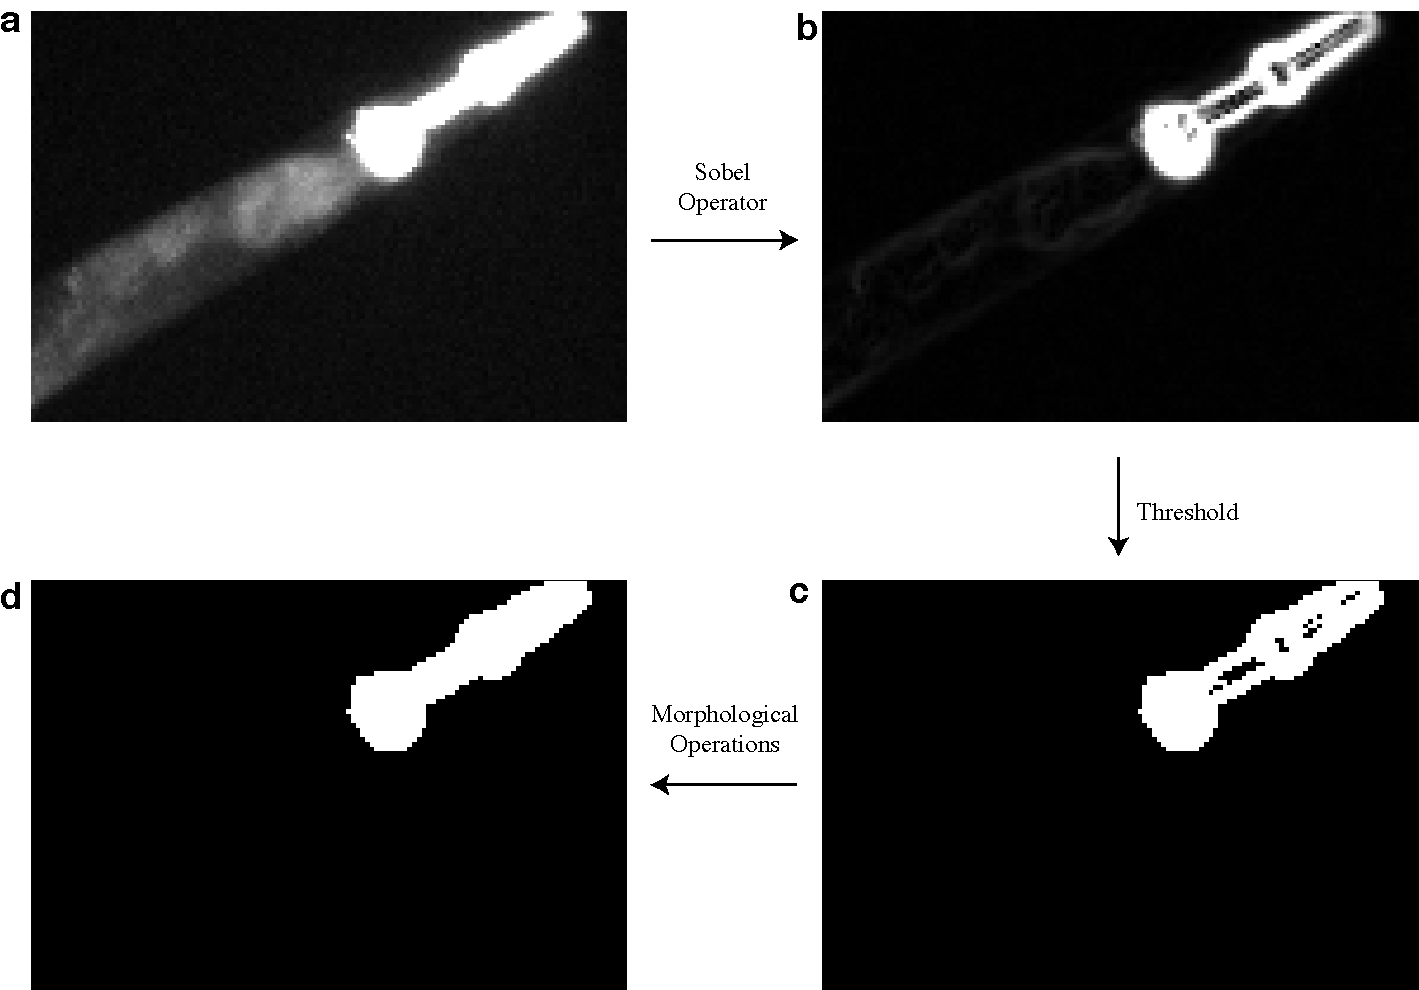
\includegraphics[scale=.40]{Figures/rendered_files/sobel}
    \decoRule
    \caption[Overview of the improved segmentation algorithm]{An overview of the improved segmentation algorithm. \textbf{a} The original image, displaying fluorescence of roGFP in the pharynx and the autofluorescence of the gut. \textbf{b} The resultant image after application of the sobel operator. \textbf{c} The resultant binary image after thresholding the edge-emphasized image. \textbf{d} The final segmented binary image, after performing morphological cleaning operations.}
    \label{fig:NewPipeline}
\end{figure}

For reasons described in \ref{TLMidlines}, an image taken with transmitted light must also be segmented. Even though the distribution of intensities in transmitted light images are very different from fluorescence images, this edge-based segmentation algorithm still performs robustly (Figure \ref{fig:TLSeg}). This highlights another benefit of the improved method: image brightness independence. If one particular genotype fluoresces dimly, an edge-based segmentation method still performs well, while the static threhsolding method requires the manual change of the threshold parameter.

\begin{figure}[ht]
    \centering
    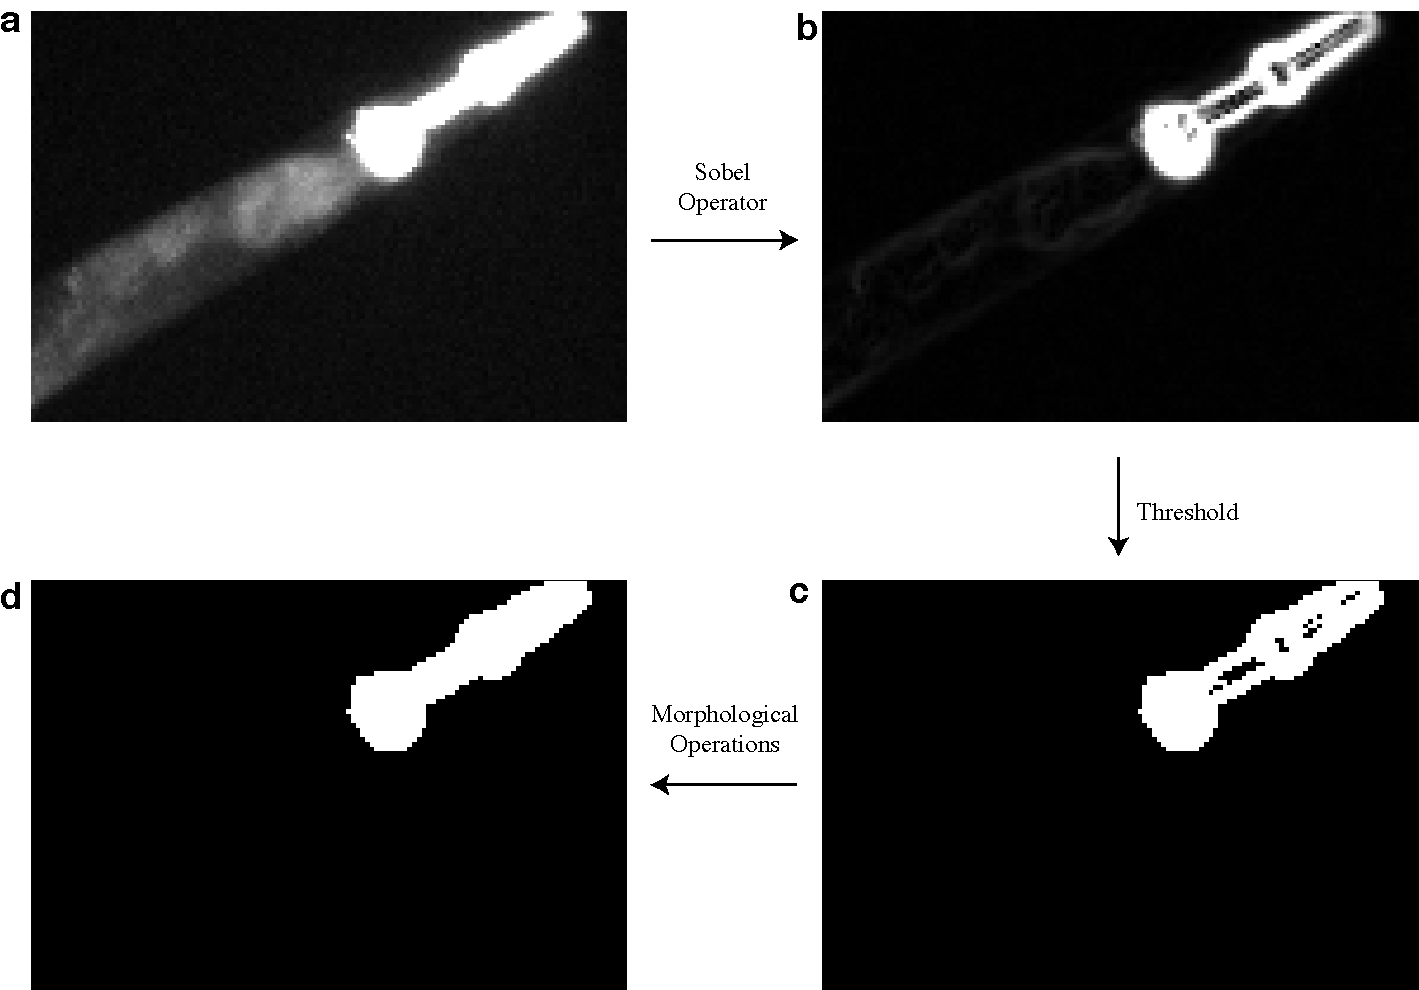
\includegraphics[scale=.40]{Figures/rendered_files/sobel}
    \decoRule
    \caption[Overview of the improved segmentation algorithm]{This should be an image of transmitted light before/after segmentation.}
    \label{fig:TLSeg}
\end{figure}

%-------------------------------------------------------------------------------------
%	SECTION 2
%-------------------------------------------------------------------------------------
\section{Flexible measurement boundaries account for anterior-posterior movment} \label{channelSegmentation}

As described in \ref{limitations}, interframe movement is a large source of error. To understand why, consider the how the previous pipeline takes measurements. First, a single mask using the image taken at 410nm is computed. This mask is then applied to both the 410nm and 470nm images. Pixels corresponding to \texttt{1} in the mask retain their value while pixels corresponding to \texttt{0} in the mask are assigned the value \texttt{0}. Measurements are taken of the masked images. Thus, if the animal pumps, measuremnt might start in the gut or halfway through the posterior bulb, depending on if the animal contracted during the first or second frame. If the animal contracts during the first frame and extends in the second, the mask will be too "short" and measurement in the second frame will start in the middle of the posterior bulb. If the animal is extended in the first frame and contracts in the second, the mask will be too "long" and measurement in the second frame will start in the gut. This error is accounted for via visual inspection of ratio images so as to exclude those animals who have moved from analysis.

\begin{figure}[ht]
    \centering
    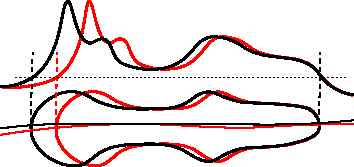
\includegraphics[scale=1.20]{Figures/rendered_files/new_boundaries_cartoon}
    \decoRule
    \caption[Flexible measurement boundaries]{A cartoon depicting the flexible measurement boundaries in the revised measurement pipeline}
    \label{fig:NewBoundariesCartoon}
\end{figure}

The new approach (summarized graphically in Figure \ref{fig:NewBoundariesCartoon}) tries to account for this movement without the need for manual exclusion. Here, segmentation masks are not applied to the images before measurement as before. Instead, they are used only in the calculation of the midlines (described in \ref{Midlines}). Intensity profiles of the unmasked images are taken under the midlines. The intensity profiles are trimmed to the point where they cross a threshold then resized to the same length via linear interpolation. Allowing measurement boundaries to move flexibly is a simple yet effective change in reducing error introduced by inter-frame pharyngeal contractions.

%-------------------------------------------------------------------------------------
%	SECTION 3
%-------------------------------------------------------------------------------------
\section{Midlines} \label{Midlines}

The previous centerline estimation algorithm takes as input an image of the segmented pharynx aligned horizontally along its anterior posterior axis and works as follows (depicted in figure \ref{fig:oldMidline}).

\begin{figure}[ht]
    \centering
    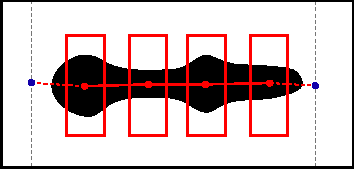
\includegraphics[scale=1.5]{Figures/rendered_files/old_midline_algorithm}
    \decoRule
    \caption[Previous centerline estimation algorithm]{Cartoon representation of the previous centerline estimation algorithm.}
    \label{fig:oldMidline}
\end{figure}

Boxes are drawn at specific static coordinates. The centroid of each shape is calculated (red points). Lines (solid) connect these points. The y-coordinates of the terminating points (blue) are determined via the point-slope method $y=mx+b$ where $m$ is the inverse of the slope of the neighboring line, $x$ is a fixed constant and $b$ is the y-coordinate of the neighboring point.


\subsection{A transmitted light image helps to anchor the midlines} \label{TLMidlines}
A major problem faced by the current centerline estimation algorithm is instability around the posterior bulb. Small positional changes in the neighboring points cause the terminal point to move dramatically. These instabilities must be manually corrected.

To address this concern, the new centerline estimation algorithm incorporates positional information from a transmitted-light image. The entire body of the worm is visible in transmitted light. We segment the transmitted light image with the algorithm described in \ref{segMethod}, resulting in a binary mask. This mask is combined with the pharyngeal mask by cuting off the transmitted-light mask when the pharyngeal mask starts. It is this combined mask that is fed into the centerline estimation algorithm. The points from the transmitted-light mask serve to constrain and anchor the previously unstable posterior-bulb region of the estimated centerline.

\subsection{A spline-based centerline algorithm improves quality around the tip}
The centerline estimation around the tip of the pharynx is subject to instabilities for similar reasons as discussed in \ref{TLMidlines}. In this case, the transmitted-light frame does not help as the body of the worm does not extend past the pharynx. To address this tip instability, a new centerline estimation algorithm was created.

The method takes as input a binary image created via the methods described in \ref{TLMidlines}. Pixels with the value \texttt{1} are treated as points in 2D space. A smoothing B-spline is fit to these points, resulting in a continuous function. Spline parameters were chosen by visual inspection.

\subsection{Dorsal-ventral tip movement is addressed with frame-specific midlines} \label{frameSpecificMidlines}
We saw in \ref{channelSegmentation} a strategy to combat the major mode of inter-frame movement, contractions of the posterior bulb. However, there is another less common mode: dorsal-ventral movement of the tip. The spline algorithm described above allows the centerline to follow the curve of the tip without human intervention. To address inter-frame movement, the new pipeline draws a midline independently in each frame. These frame-specific midlines are used to take profile measurements.

%-------------------------------------------------------------------------------------
%	SECTION 4
%-------------------------------------------------------------------------------------
\section{Channel Registration picks up the slack}

The frame-specific midline approach discussed in \ref{frameSpecificMidlines} introduces problems of its own. Specifically, the length of the measurement vector may be stretched nonlinearly due to differences in the arc length of each midline. That is, some sections of the intensity profile measured under these lines might be stretched while others are compressed. To approach these nonlinear stretches and compressions, we utilized a functionalized version of the dynamic time warping algorithm.

\todo[inline]{explanation of fda registration} 
%% Chapter Template

\chapter{Results} % Main chapter title

\label{Chapter3} % Change X to a consecutive number; for referencing this chapter elsewhere, use \ref{ChapterX}

%-------------------------------------------------------------------------------------
%	SECTION 1
%-------------------------------------------------------------------------------------
\section{Definition of Error}
To assess the degree to which changes in the analysis pipeline affect the quality of measurement, a definition of error must first be decided upon. Error ($\epsilon$) is defined to be a function over pharynx space ($p$) which is the difference between the intensity measured in one frame and another. The difference is normalized by the average intensity of the two frames at 410 nm.


\[\epsilon(p) = \frac{I_{410_1}(p) - I_{410_2}(p)}{\frac{I_{410_1}(p) + I_{410_2}(p)}{2}}\]

To calculate redox potentials, we take the first frame at 410 nm and the second at 470 nm. When we quantify error, however, we must use a single wavelength as the changes in emission spectra would confound the errors.

%-------------------------------------------------------------------------------------
%	SECTION 2
%-------------------------------------------------------------------------------------
\section{Collection of test data} \label{testCollection}

A large number of technical replicates were collected. A single animal was plated on 5.5 mM levamisole and imaged 57 times in pairs of two images both at 410 nm. A paired-sample t-test indicates no significant difference (p=0.41) between the first and second intensity profile.

\begin{figure}[ht]
    \centering
    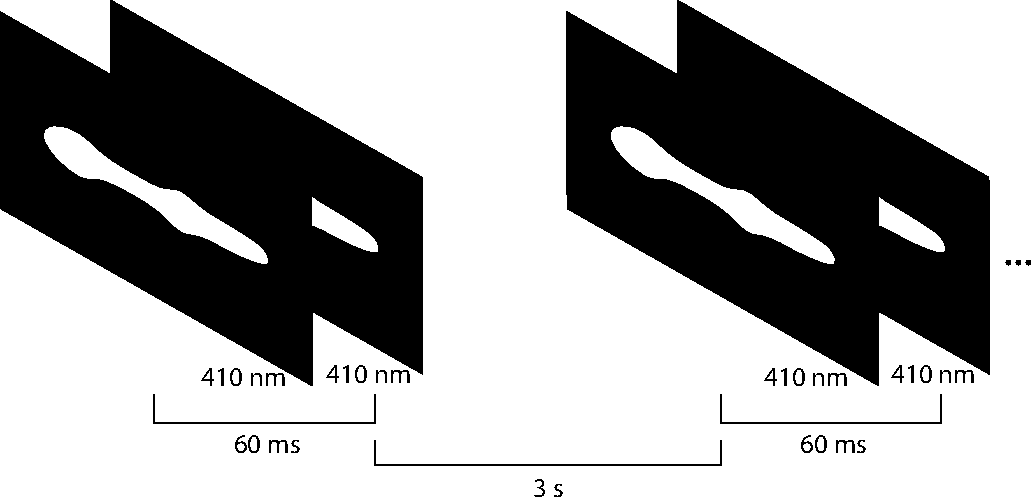
\includegraphics[scale=0.8]{Figures/rendered_files/test_imaging_schematic}
    \decoRule
    \caption[Test imaging schematic]{}
    \label{fig:TestImagingSchematic}
\end{figure}

A set of ratiometric images (collection described in \ref{testCollection}) was hand-classified according to the degree of movement (0 - 3) in four regions: the posterior bulb, anterior bulb, sides of the tip, and tip. Figure \ref{fig:RPosteriorMovement} shows the mean $I_{410}/I_{410}$ measured under the midline and colored by degree of movement in the posterior bulb. A ratio of 1 indicates no error.

\begin{figure}[ht]
    \centering
    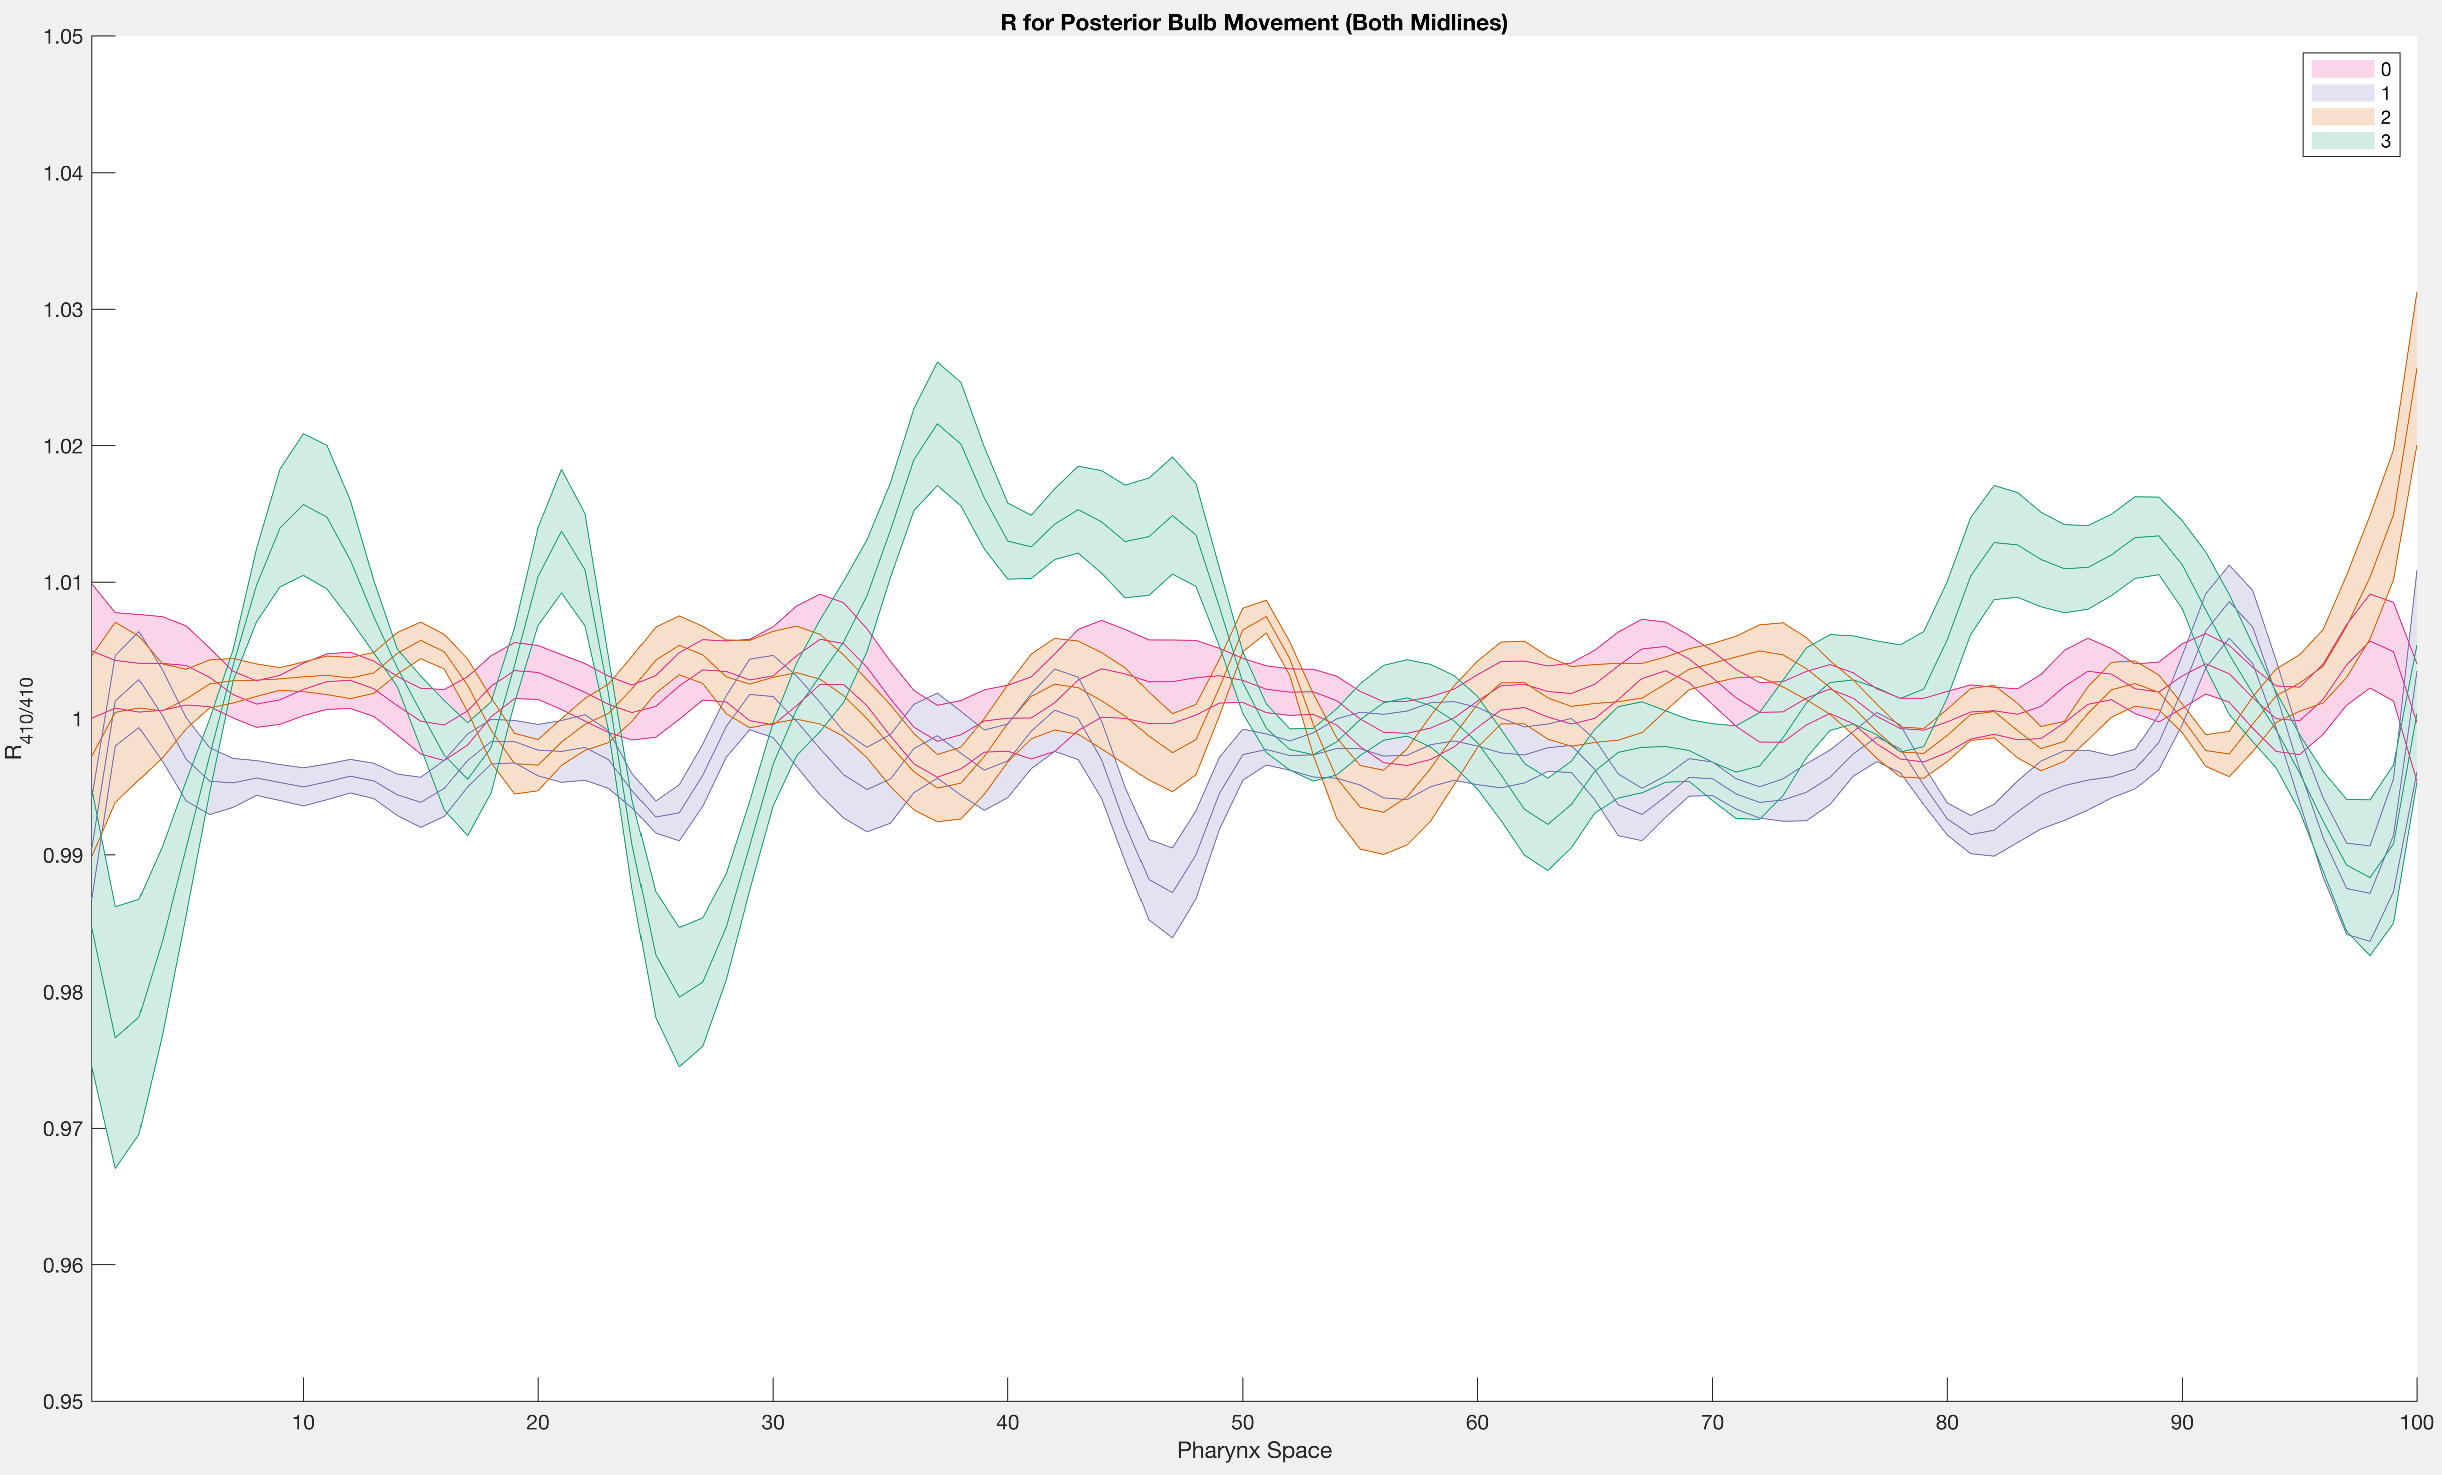
\includegraphics[scale=0.25]{Figures/rendered_files/R_posterior_movement}
    \decoRule
    \caption[Error by strategy in the natural data set]{Relative error}
    \label{fig:RPosteriorMovement}
\end{figure}

%-------------------------------------------------------------------------------------
%	SECTION 3
%-------------------------------------------------------------------------------------
\section{A partially synthetic data set increases statistical power}

Instead of comparing pairs of measurements taken back-to-back, we can compare all possible pairs. Given n images, we generate ${n \choose 2} = \frac{n!}{2!(n-2)!}$ pairs. However, repeated excitation seems to attenuate the emission amplitude of the sensor (Figure \ref{fig:AvgIntensityOverTime}). To account for this effect (known as photobleaching) we generate pairs starting at the 15th imaged pair and exclude outliers (Figure \ref{fig:AvgIntensityOverTime}).

\begin{figure}[ht]
    \centering
    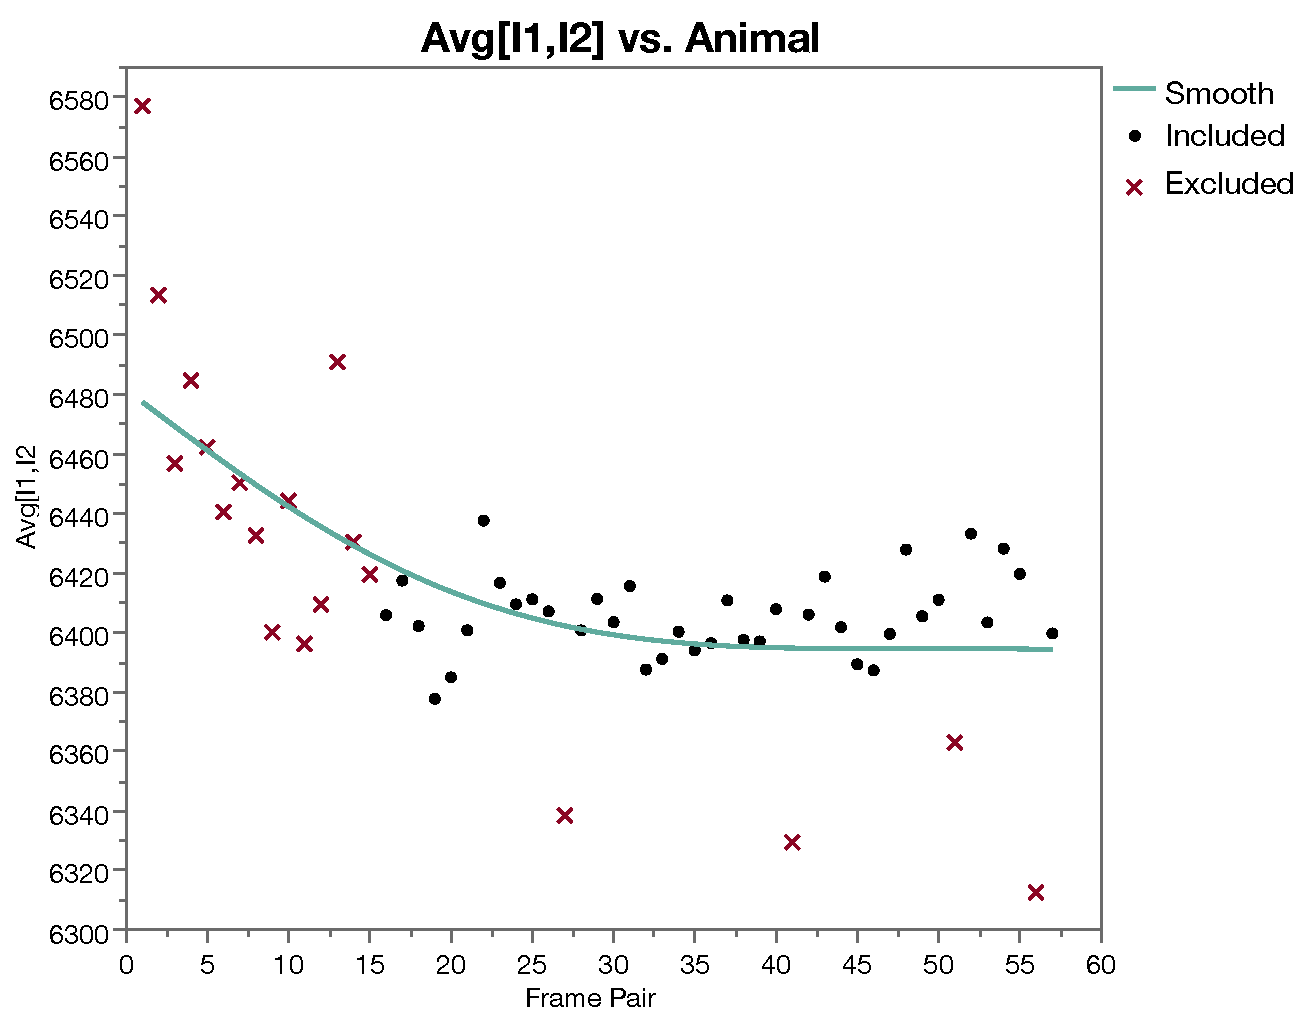
\includegraphics[scale=0.35]{Figures/rendered_files/photobleaching}
    \decoRule
    \caption[Average intensity over time in technical replicates]{The average intensity over time in technical replicates. Red xs mark image pairs excluded from the recombination.}
    \label{fig:AvgIntensityOverTime}
\end{figure}

Since the average time between frames in this synthetic data set is 10 seconds\todo{do this calculation}, there is a large degree of inter-frame movement. Because the true test data has only 12 \todo{real number} pairs which display inter-frame movement, this partially synthetic data set allows us to be more confident about the changes in error seen using different analysis strategies.


%-------------------------------------------------------------------------------------
%	SECTION 4
%-------------------------------------------------------------------------------------
\section{Reductions in Manual Intervention}

\subsection{Incorporation of edge information increases segmentation accuracy}

To compare the accuracy of segmentation methods, we first create a "gold-standard" set of images which were segmented by hand to ensure accuracy. The segmentation methods were applied to the same set of images and the resultant masks were compared via the total difference measure described in Yang et al. (A Supervised Approach to the Evaluation of Image Segmentation Methods).

\todo[inline]{show figures comparing \% requiring manual intervention for segmentation and for midlines}

\subsection{Incorporation of transmitted-light information increases centerline stability around the posterior bulb}

To compare the stability of the centerline around the posterior bulb, we 

%-------------------------------------------------------------------------------------
%	SECTION 5
%-------------------------------------------------------------------------------------
\section{Channel-Specific Masks and Midlines Reduce Error}

% \begin{figure}[ht]
%     \centering
%     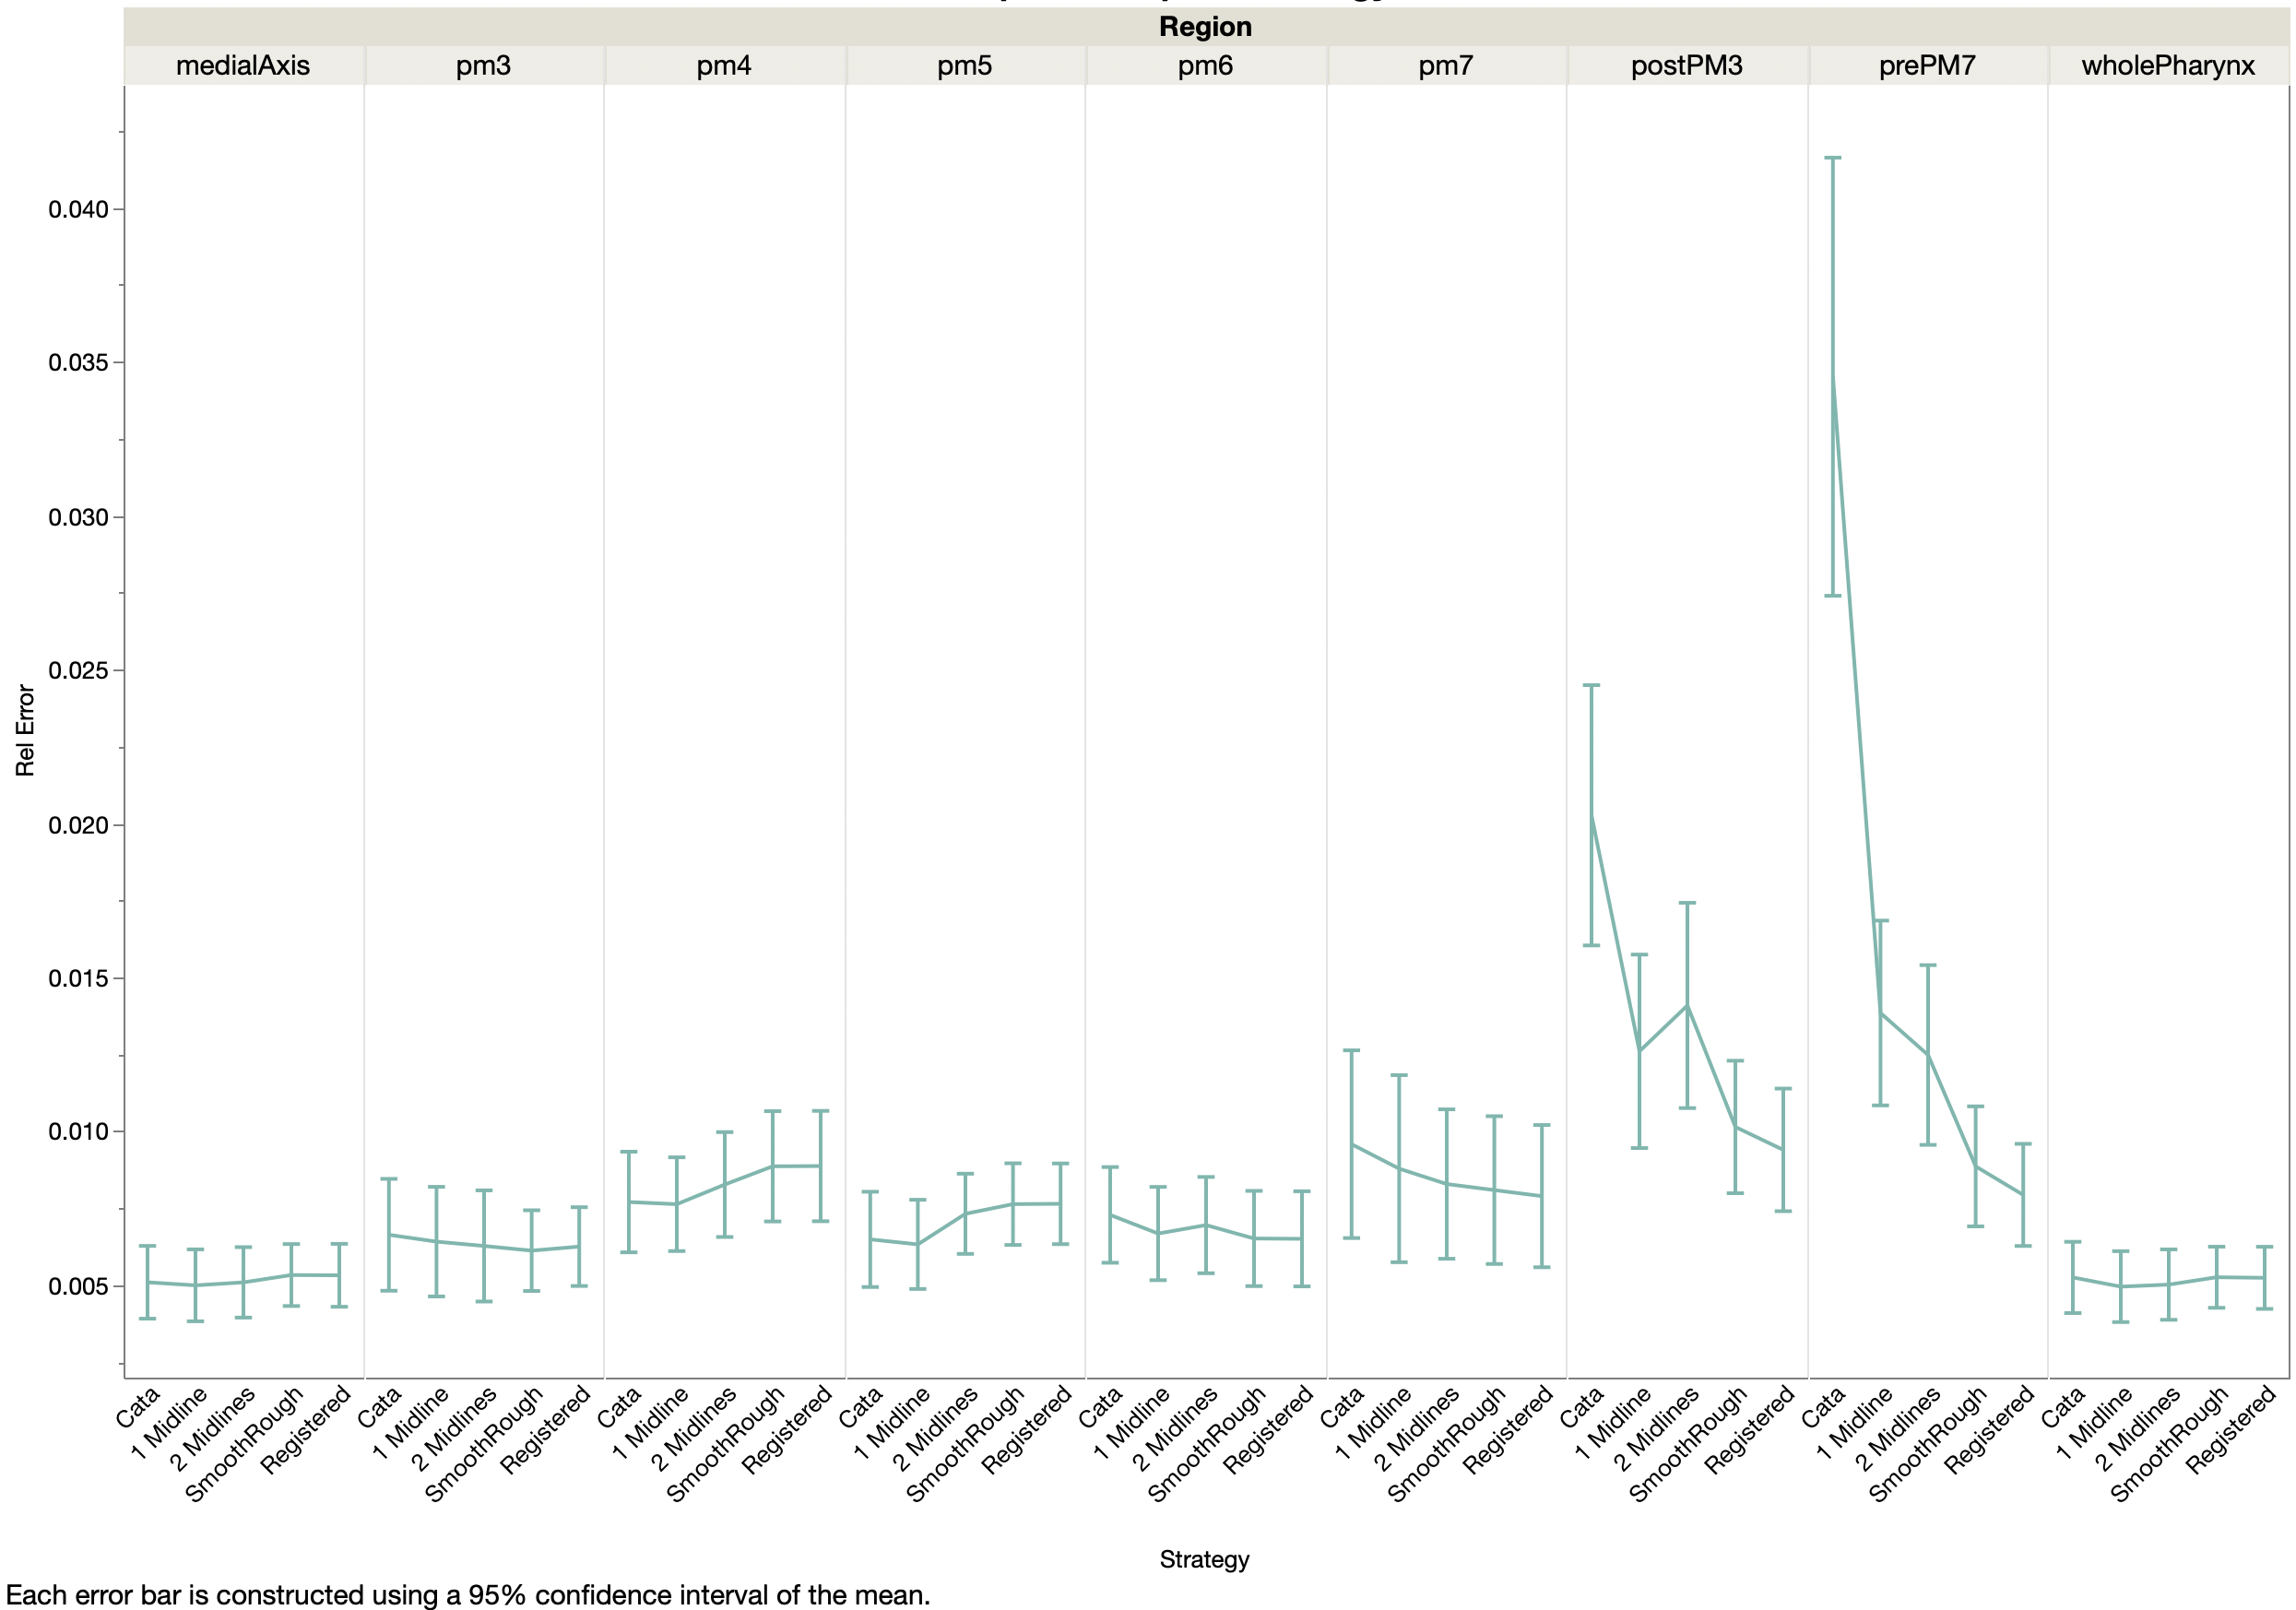
\includegraphics[scale=0.15]{Figures/rendered_files/error_by_strategy_natural}
%     \decoRule
%     \caption[Error by strategy in the natural data set]{Relative error}
%     \label{fig:PercentErrorNatural}
% \end{figure}

\begin{figure}[ht]
    \centering
    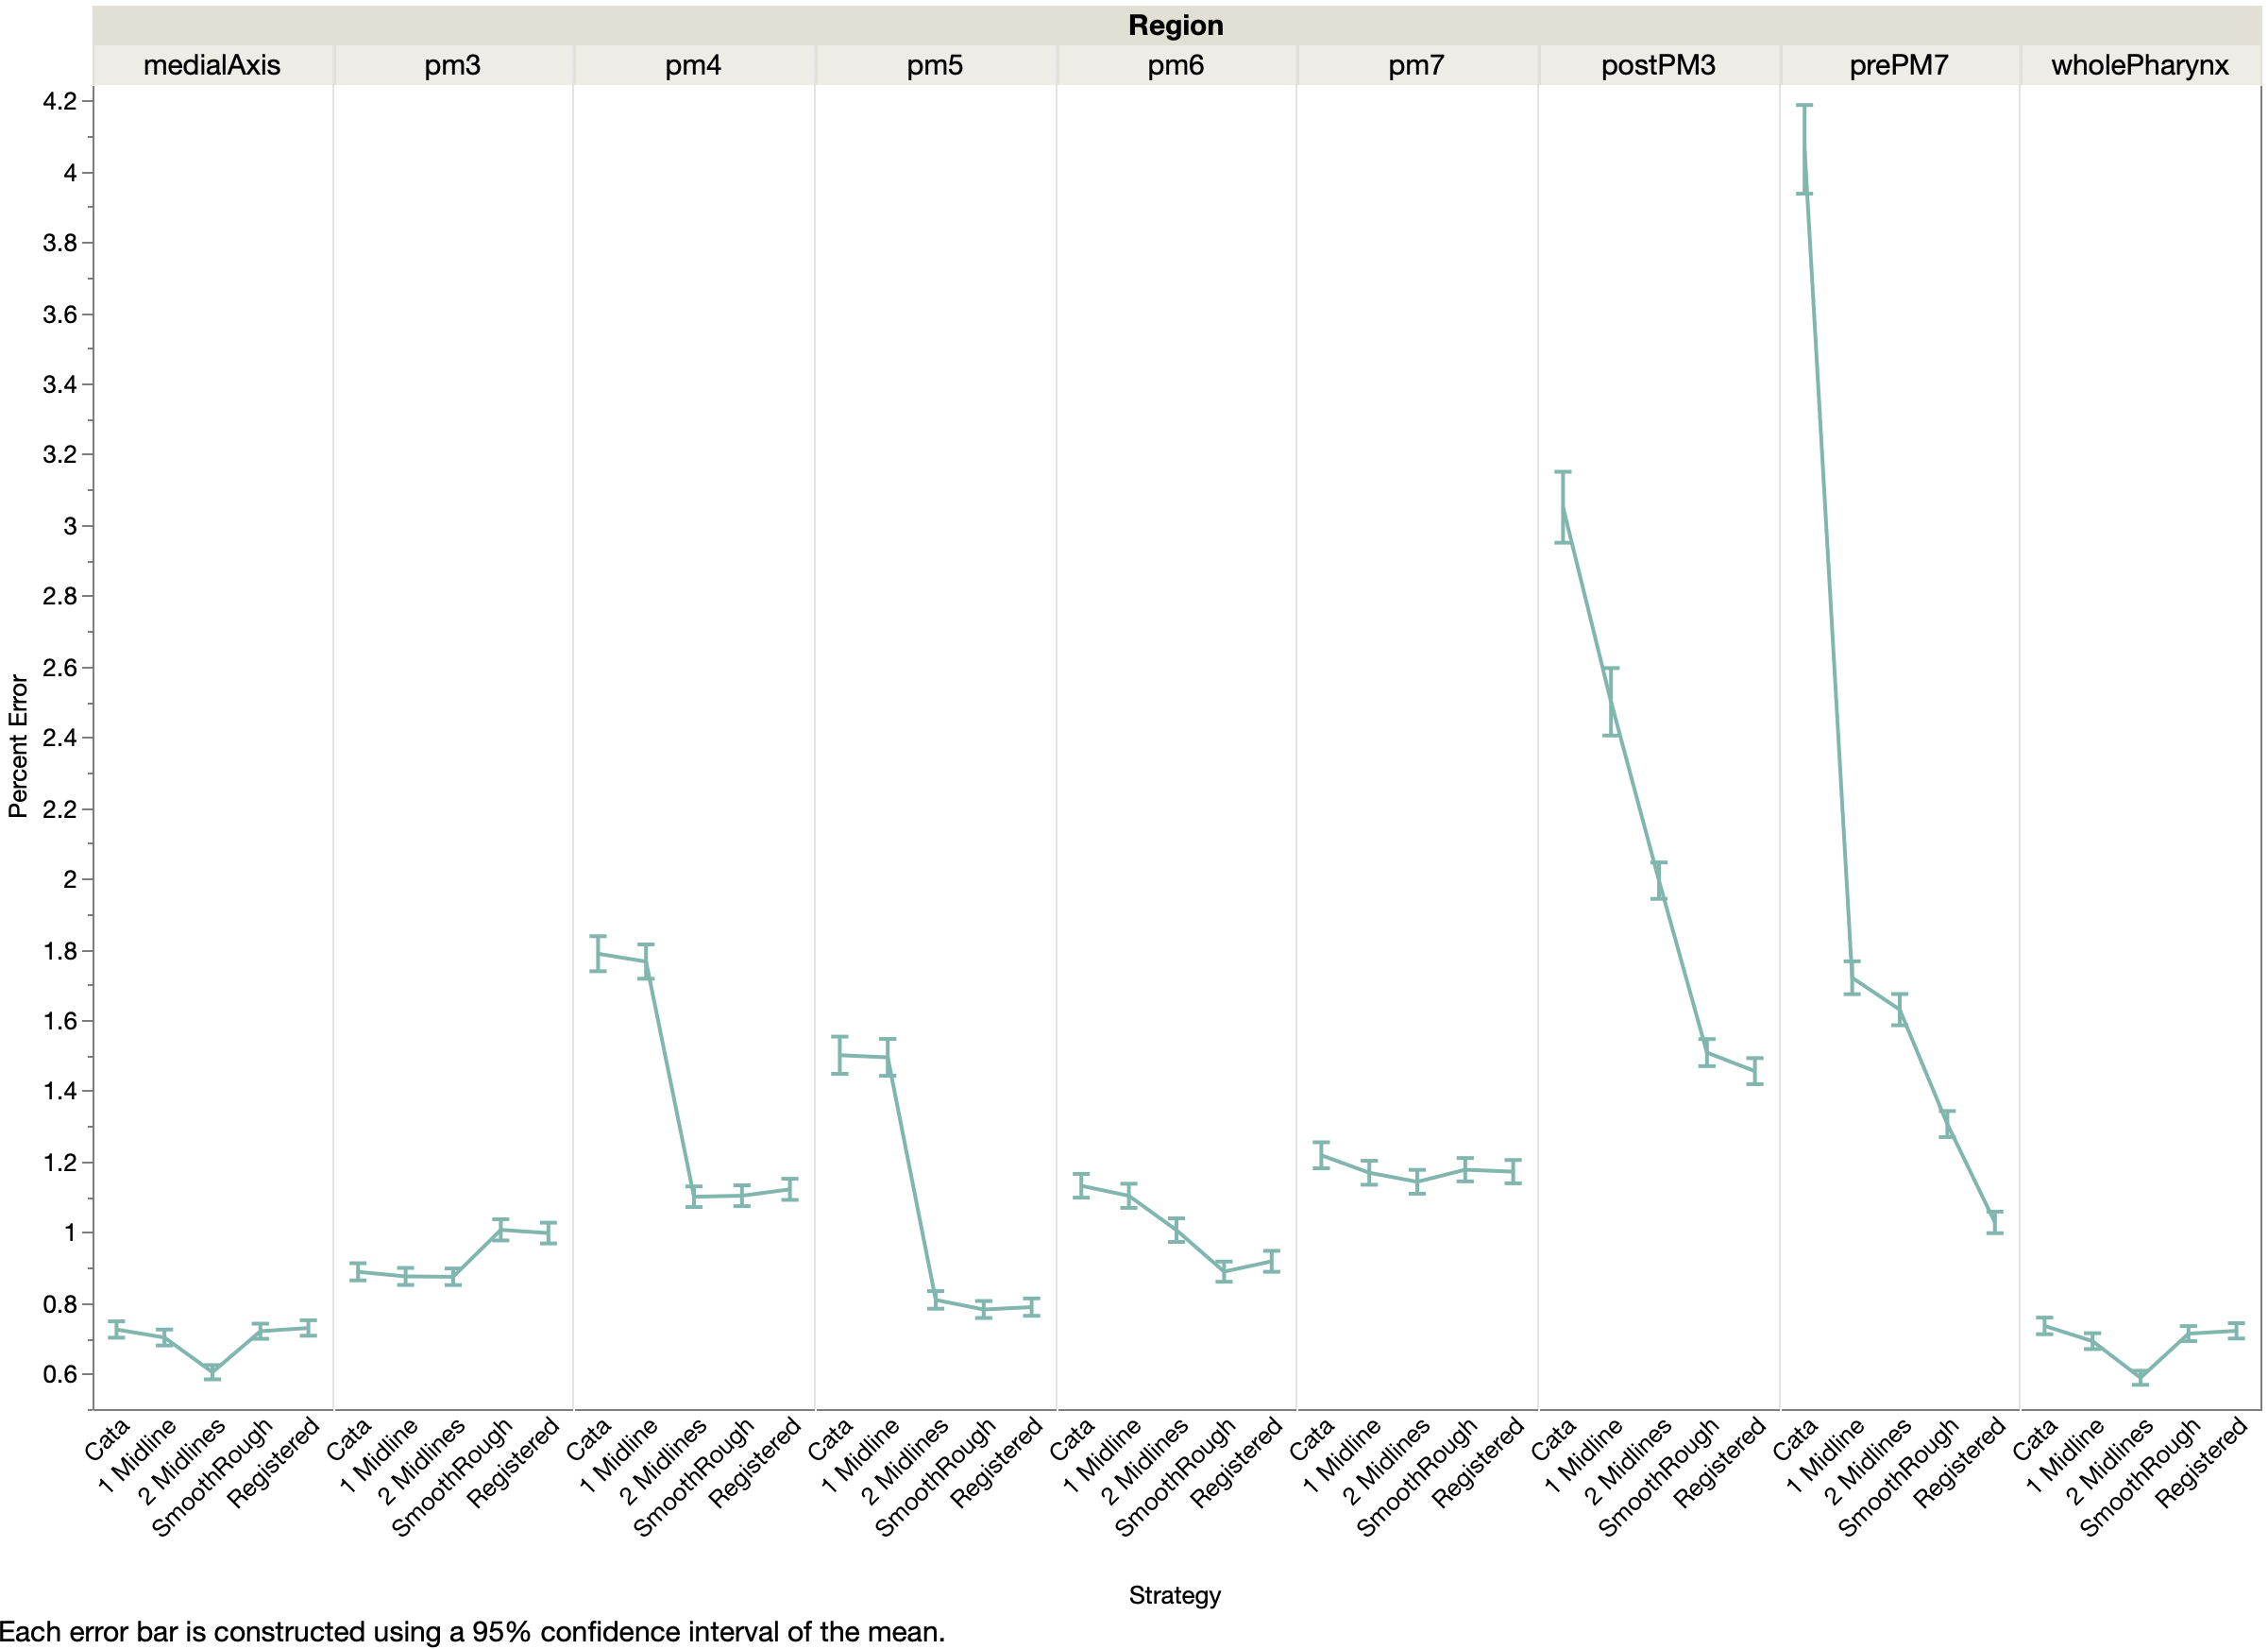
\includegraphics[scale=0.15]{Figures/rendered_files/error_by_strategy_synthetic}
    \decoRule
    \caption[Error by strategy in the synthetic data set]{}
    \label{fig:PercentErrorSynthetic}
\end{figure}
%\chapter{Discussion}

\label{Chapter4}

Genetically encoded redox-sensitive fluorescent biomarkers have spurred a revolution in the study of dynamic cellular redox processes. While the ratiometric nature of these sensors yields many desirable qualities, it also necessitates careful analysis in the event of inter-frame movement. 

This thesis has introduced how inter-frame movement introduces error in ratiometric fluorescent microscopy and proposed three strategies to mitigate this error in the context of the pharyngeal muscle of the nematode \textit{C. elegans}. Frame-specific masks allow for flexible measurement boundaries, which achieves a limited form of global linear registration. Frame-specific midlines account for the dorsoventral movement common at the anterior regions of the pharynx. A functional approach to registration accounts for the differences in arc-length of the frame-specific midlines, and achieves the non-linear registration that frame-specific midlines require. These improvements allow previously unusable data to be re-analyzed and will require fewer animals to be excluded in future experiments.

This thesis has also shown how new approaches to segmentation and centerline estimation reduces the need for manual input in the pipeline via incorporation of edge information and transmitted-light information, respectively. In most cases, the pipeline requires no manual input and analysis can be done with little effort and time, increasing experimental throughput.

%-------------------------------------------------------------------------------------
%	SECTION 1
%-------------------------------------------------------------------------------------
\section{Future Directions}

% SUBSECTION
\subsection{Automatic movement detection}

This thesis has focused on the mitigation of the error introduced by inter-frame movement. As noted, not all error can be removed by these methods. As such, it would be useful for an automated classification system to detect inter-frame movement. The fundamental difficulty with this task is that in an experimental setting the image pairs consist of one image at 410 nm and another at 470 nm. Because the excitation spectra of roGFP is different at each wavelength, it is difficult to determine if the differences in each image's intensity profile is due to movement or true biochemical activity. This concern could be addressed by quantifying distance between midlines instead of difference in intensity profile. Alternatively, different imaging strategies could be developed. For example, if four images were taken of each animal at alternating excitation wavelengths, differences in the pairs with the same wavelength could be used to quantify error and thereby inter-frame movement.

% SUBSECTION
\subsection{Extension to different tissues}

The analysis pipeline described in this thesis is highly specific to the pharyngeal muscle. Due to its stereotyped geometry, this tissue has been an ideal foundation on which to build. However, there is considerable interest in understanding dynamic redox processes in other tissues such as the intestine and nervous system. Each tissue will surely introduce its own challenges that will need to be individually addressed. Precise methodologies for quantifying redox processes in these different tissues will lead to a deeper understanding of how these processes are regulated at an organismal level.

%-------------------------------------------------------------------------------------
%	SECTION 2
%-------------------------------------------------------------------------------------
 
%\include{Chapters/Chapter5} 

%----------------------------------------------------------------------------------------
%	THESIS CONTENT - APPENDICES
%----------------------------------------------------------------------------------------

\appendix % Cue to tell LaTeX that the following "chapters" are Appendices

% Include the appendices of the thesis as separate files from the Appendices folder
% Uncomment the lines as you write the Appendices

% Appendix A

\chapter{Frequently Asked Questions} % Main appendix title

\label{AppendixA} % For referencing this appendix elsewhere, use \ref{AppendixA}

\section{How do I change the colors of links?}

The color of links can be changed to your liking using:

{\small\verb!\hypersetup{urlcolor=red}!}, or

{\small\verb!\hypersetup{citecolor=green}!}, or

{\small\verb!\hypersetup{allcolor=blue}!}.

\noindent If you want to completely hide the links, you can use:

{\small\verb!\hypersetup{allcolors=.}!}, or even better: 

{\small\verb!\hypersetup{hidelinks}!}.

\noindent If you want to have obvious links in the PDF but not the printed text, use:

{\small\verb!\hypersetup{colorlinks=false}!}.

%\include{Appendices/AppendixB}
%\include{Appendices/AppendixC}

%----------------------------------------------------------------------------------------
%	BIBLIOGRAPHY
%----------------------------------------------------------------------------------------

\printbibliography[heading=bibintoc]

%----------------------------------------------------------------------------------------

\end{document}  
